\documentclass[11pt,a4paper]{article}
\usepackage[margin=2.2cm]{geometry}
\usepackage{graphicx}
\usepackage{booktabs}
\usepackage{amsmath}
\usepackage[colorlinks=true,linkcolor=blue,urlcolor=blue]{hyperref}
\graphicspath{{mesh_report_figs/}}

\title{Mesh charge-injection timing study\\
\large n\_TOF X17 Micromegas $\gamma$-flash countermeasure --- delay scan and retiming}
\author{X17 DAQ (automated study)}
\date{2026-07-11}

\begin{document}
\maketitle

\begin{abstract}
The prompt $\gamma$-flash saturates the Micromegas detectors at every proton
pulse. A charge-injection pulse applied to the detector meshes
(Module~6 section~B of the N1081B trigger crate) is meant to counteract it,
but was found firing $\sim$760\,ns \emph{before} the flash, with no overlap.
We scanned the injection delay using flash-triggered DREAM runs and found
that placing the injection $\sim$180\,ns before the flash rise suppresses
the event-averaged flash amplitude on detector~C by $\sim$45\%, while an
injection arriving exactly at the rise gives no suppression. The delay knob
(M6.B in0 Gate\&Delay) was retimed from 500\,ns to \textbf{1260\,ns}.
\end{abstract}

\section{Setup and method}

\paragraph{Injection chain.} PS/T0 $\rightarrow$ M6 (.245) section~B fanout
$\rightarrow$ four outputs (500\,ns monostable) $\rightarrow$ Micromegas
meshes. The timing knob is the \textbf{input Gate\&Delay of M6.B channel~0}
(\texttt{gate}=50\,ns, \texttt{delay}=the scanned parameter; 5\,ns steps).
The injected pulse rails detector~A's front-end, couples moderately to
B/C, and is therefore directly visible in the DREAM waveforms.

\paragraph{Measurement.} Flash-triggered DREAM runs (run mode~1:
M4.D=OR(lemo0)=PS line; 400~samples $\times$ 20\,ns, latency~60;
$\sim$79 events per 4\,min at the parasitic pulse rate). For each delay
setting the event-averaged, channel-averaged waveform per FEU
(\texttt{check\_flash.py} profiles) gives the flash amplitude and the
injection position. FEU$\to$detector map: A=03/04, B=05/06, C=07/08,
D=01/02 ($x$,$y$).

\paragraph{Runs.}
\begin{center}
\begin{tabular}{lllcc}
\toprule
variant & M6.B in0 delay & time (2026-07-11) & pulses used & $\langle I\rangle$ [$10^{10}$\,p] \\
\midrule
\texttt{m1\_lat60}        & 500\,ns (original) & 12:35 & 89  & 675 \\
\texttt{m6\_inj\_aligned}  & 1260\,ns           & 15:48 & 130 & 627 \\
\texttt{m6\_inj\_aligned2} & 1440\,ns           & 15:55 & 95  & 633 \\
\bottomrule
\end{tabular}
\end{center}
The two decisive runs (1260 vs.\ 1440\,ns) had beam intensities within 1\%
of each other, so the amplitude difference below cannot be a beam effect.

\section{Results}

\noindent Detector-C flash amplitude (event-averaged peak $-$ baseline,
FEU~07) vs.\ injection delay:
\begin{center}
\begin{tabular}{lccc}
\toprule
M6.B in0 delay & injection vs.\ flash rise & det~C peak$-$base [ADC] & change \\
\midrule
500\,ns (original) & $\sim$760\,ns early, separate pulse & 3099 & --- \\
\textbf{1260\,ns (chosen)} & $\sim$180\,ns before the rise & \textbf{1709} & \textbf{$-$45\%} \\
1440\,ns & at/just after the rise & 3312 & $+7\%$ \\
\bottomrule
\end{tabular}
\end{center}
Figures~\ref{fig:profiles}--\ref{fig:peaks} show the underlying waveforms.

\begin{figure}[p]
\centering
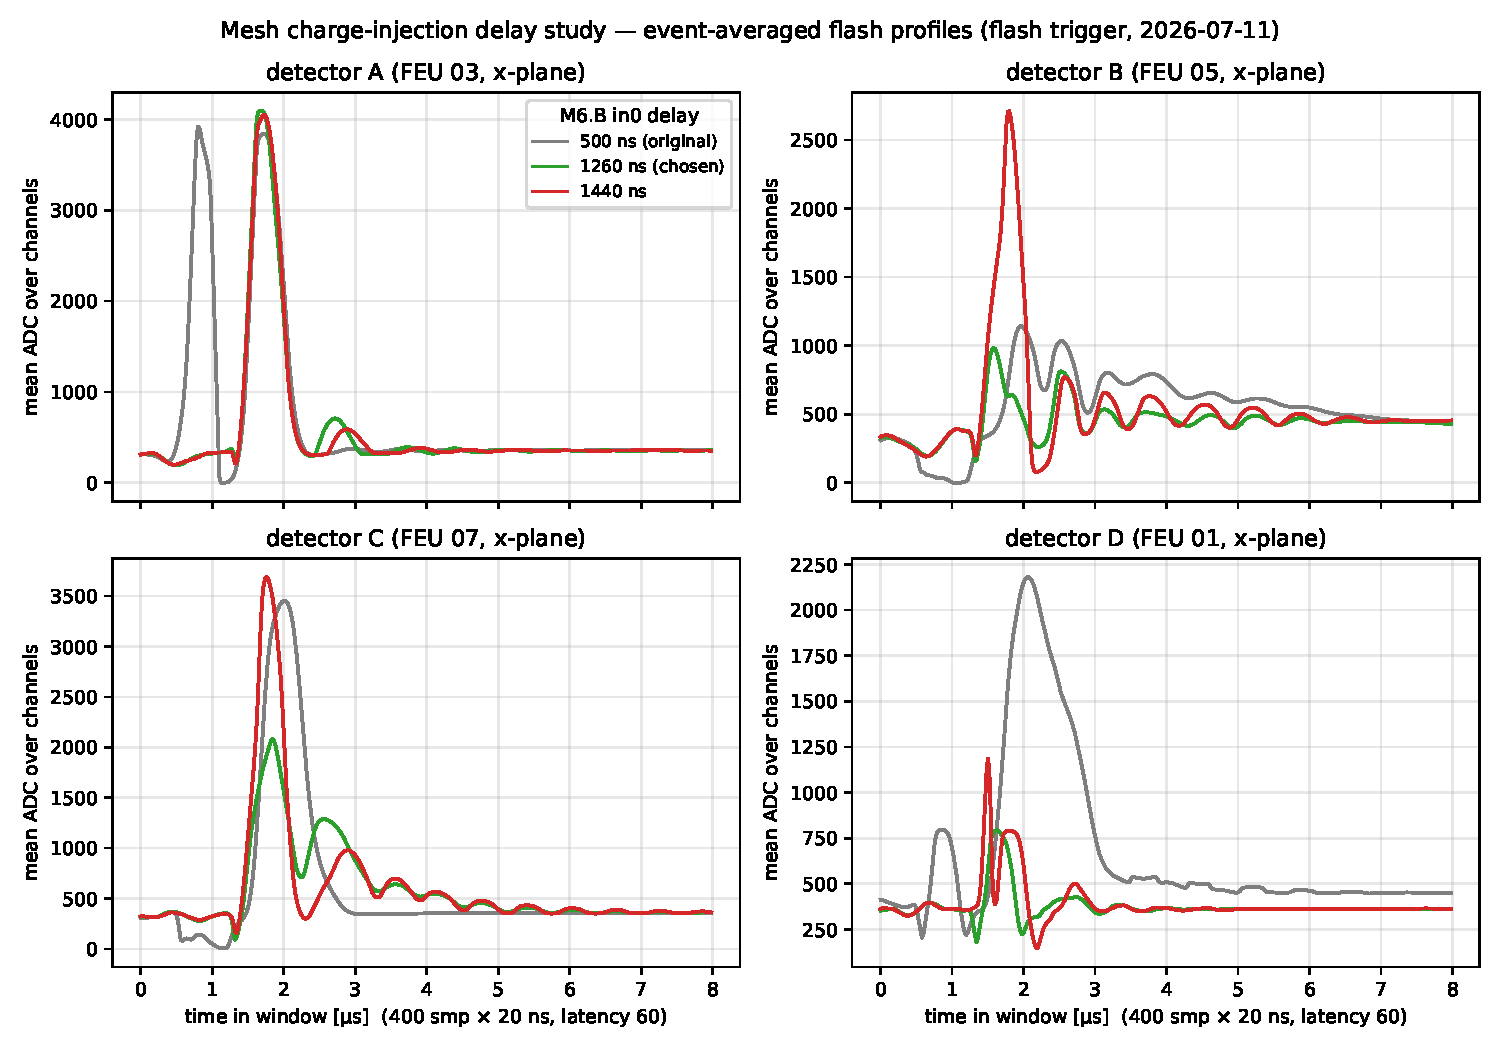
\includegraphics[width=\textwidth]{mesh_fig_profiles}
\caption{\label{fig:profiles}Event-averaged, channel-averaged waveforms per detector for the
three delay settings. Gray: original 500\,ns --- the injection is the
separate railed pulse at $\sim$0.8\,\textmu s, the flash follows at
$\sim$1.6--2\,\textmu s. Green: 1260\,ns --- injection merged into the flash
rise; detector~C's flash peak drops by 45\%. Red: 1440\,ns --- injection at
the rise; no suppression (det~C), and detector~B's peak is
\emph{enhanced} (constructive overlap). Detector~A rails at 4095 in all
settings (strongest injection coupling). \textbf{Caveat:} the detector-D
panel is not comparable across runs --- its amplification HV was 640\,V
during the 500\,ns run and 100\,V (parked after a trip) during the other
two.}
\end{figure}

\begin{figure}[p]
\centering
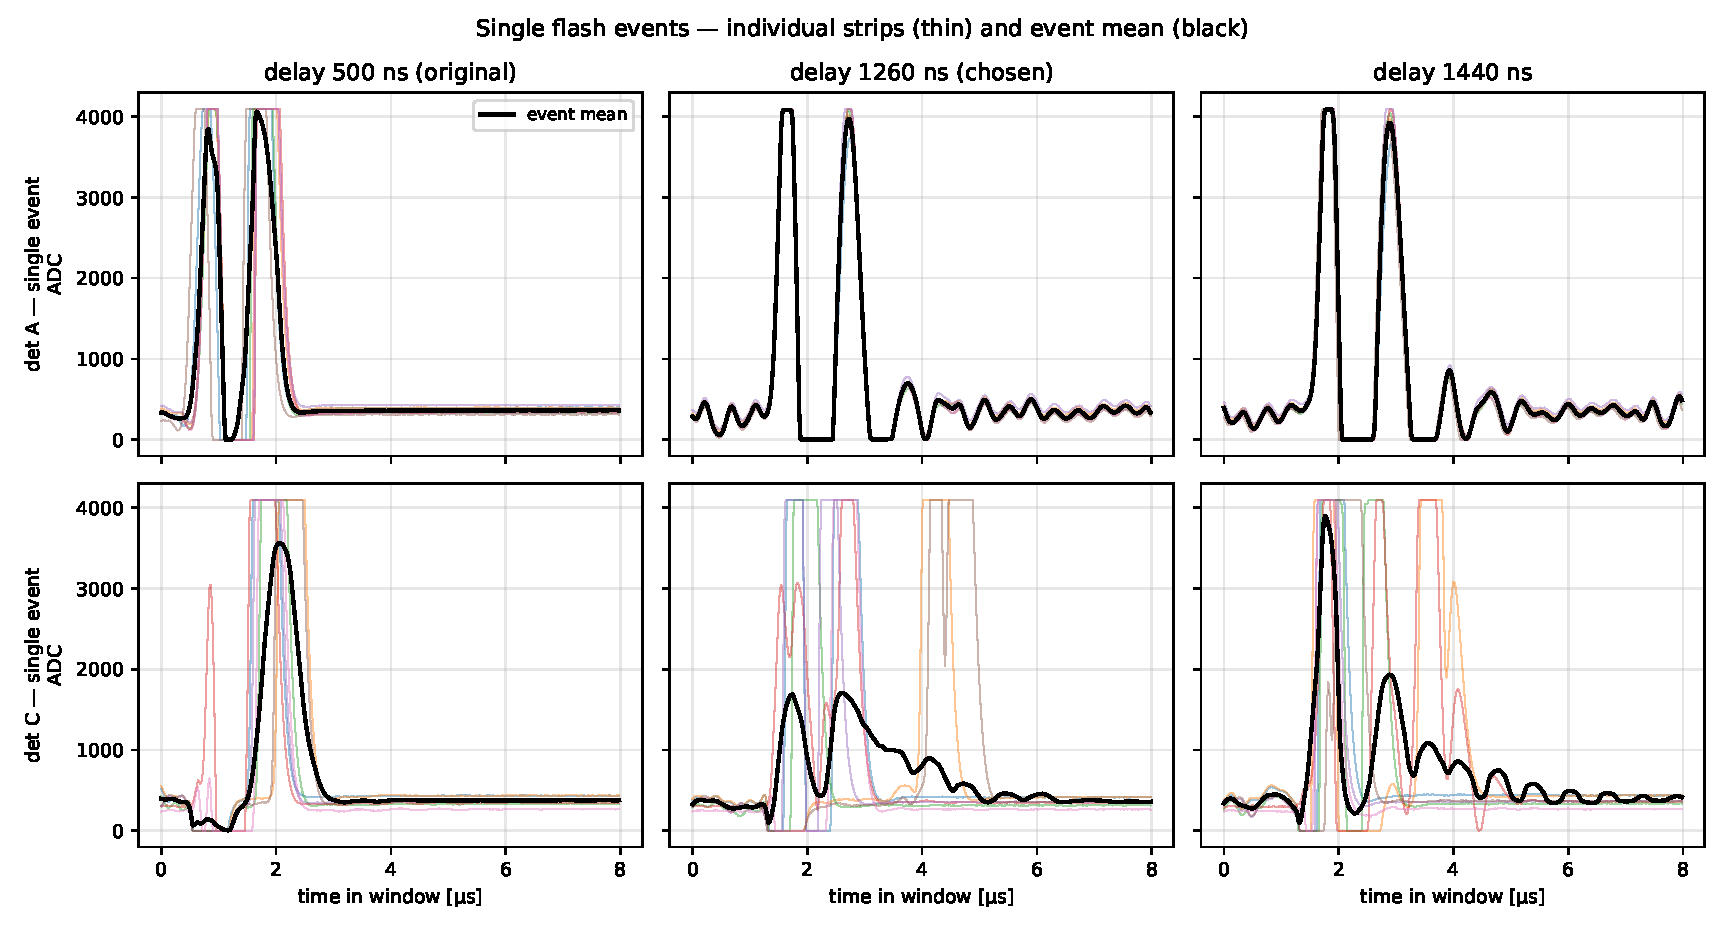
\includegraphics[width=\textwidth]{mesh_fig_events}
\caption{\label{fig:events}Single flash events (detectors A and C): individual strips (thin,
subset) and the event mean (black). At 500\,ns detector~A shows the two
separate railed pulses (injection, then flash). At 1260/1440\,ns they merge.
The hard clips to ADC~0 are the coherent post-pulse undershoot.}
\end{figure}

\begin{figure}[h]
\centering
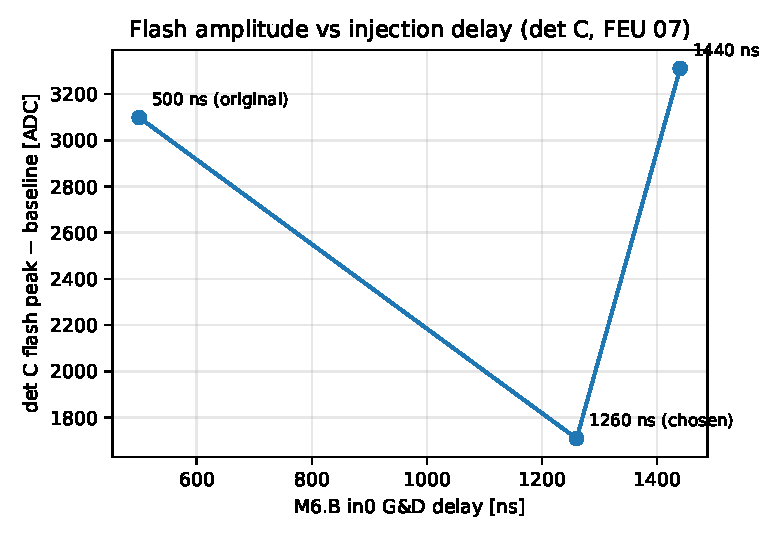
\includegraphics[width=0.62\textwidth]{mesh_fig_peaks}
\caption{\label{fig:peaks}Detector-C event-averaged flash amplitude vs.\ injection delay.}
\end{figure}

\section{Interpretation and recommendation}

\begin{itemize}
\item The cancellation needs the mesh to be \emph{pre-loaded}: an injection
arriving $\sim$180\,ns \emph{before} the flash rise suppresses the recorded
flash by $\sim$45\% (det~C), whereas an injection at the rise does nothing
(det~C) or even adds constructively (det~B). ``Right at the beginning of
the flash'' is therefore best implemented as \emph{slightly before} it.
\item The response is detector-dependent (coupling and polarity differ per
mesh): A rails regardless; C benefits most; B prefers earlier injection as
well (its 1440\,ns peak nearly triples the 500\,ns one).
\item \textbf{Operating point set: M6.B in0 delay = 1260\,ns} (as-left,
snapshot \texttt{dump\_2026-07-11\_veto\_injection\_final.json}).
\item The lever arm is exactly 1\,ns per ns (input G\&D). A finer scan
(1100--1350\,ns in 50\,ns steps, one 4-min flash run each) would locate the
suppression optimum per detector; amplitudes should be normalised to the
beam intensity logged in \texttt{beam\_monitor/logs/}.
\end{itemize}

\section*{Provenance}
Runs and figures: \texttt{\~{}/beam\_july/test/latency\_singles/}
(\texttt{m1\_lat60}, \texttt{m6\_inj\_aligned}, \texttt{m6\_inj\_aligned2};
figure script \texttt{make\_mesh\_report\_figs.py}). Trigger/readout context:
\texttt{n1081b/RUN\_MODES\_2026-07.md} and
\texttt{n1081b/HANDOFF\_2026-07-11\_latency\_tuning.md}. Board state:
\texttt{n1081b/snapshots/dump\_2026-07-11\_veto\_injection\_final.json}.

\end{document}
